%defining document class
\documentclass{article}
\usepackage[utf8]{inputenc}
%setting up page layout
\usepackage{lipsum}
\usepackage[margin=1in,left=1in,includefoot]{geometry}

%Inserting package to import picture/images
\usepackage{graphicx}
% allows control of float positions
\usepackage{float} 
%header and footer
\usepackage{fancyhdr}
 
\pagestyle{fancy}
\fancyhf{}
\fancyfoot[L]{Sudip Siwakoti}
\fancyfoot[C]{\#12956936}
\fancyfoot[R]{\thepage}
\renewcommand{\headrulewidth}{0pt}

\parindent=0pt
\parskip=\medskipamount

%start compiling document
\begin{document}
% creating title page
\begin{titlepage}
%defining alingment of content
	\begin{center}
    \line(1,0){475}\\
% defining spacing    
   [2.5mm]
    \huge{\bfseries INSERT TITLE}\\
    \line(1,0){475}\\
    [3mm]
    \textsc{\Large INSERT REPORT TYPE}\\
    [6cm]
    \textsc{\small \\
    [1mm]
    31005-MACHINE LEARNING\\
    \line(1,0){150}\\
    SPRING 2019}\\
    [6.cm]
    \end{center}
% shifting alingment to left    
    \begin{flushleft}
% inserting line    
    \line(1,0){500}\\
    \textsc{\large Sudent Name: Sudip Siwakoti \\Student Number: 12956936\\ Tutorial: 9 \\ Group: 2 }
    \end{flushleft}
    \lipsum[0]
\end{titlepage}
%inserting table of content.
\tableofcontents
% removing page number form table of content
\thispagestyle{empty}
%clearing rest of the page
\cleardoublepage
%resetting page number 
\setcounter{page}{1}

%starting section and labeling section
\section{INTRODUCTION}\label{sec:intor}


We hear the word sustainability in every step of our day to day life, but what is sustainability? People seems to talk a lot about sustainability but if we carefully listen to the conversation around us, we can understand that most of the conversation on sustainability is just focused on environmental sustainability while sustainability itself is a vast term that significantly impacts every aspect of life in this universe. (Dowling et al. 2016 p. 115) quotes Tim Jackson (2010) said ‘Sustainability is the art of living well, within the ecological limits of a finite Planet.’  Sustainability also can be defined as system within which all the subsystems are in harmony with each other and none of the sub-system can exist without each other. Engineering is one of the major field that has integrated sustainability as a core value to build future.\\
\\
Past engineers have mainly focused on technical and economic feasibilities of systems design, whereas, future engineers face major challenges to incorporate  the entire spectrum of sustainability aspects (Sharifah et al. 2014).  Economic, environmental, and social sustainability are 3 key aspect of sustainable engineering and address multi-generational dimension.

%starting new section
\section{ASPECTS OF SUSTAINABILITY}
\subsection{Environmental Sustainability}\label{SEC:Enviro}
The term environment broadly applies to all the natural and build environment on this planet. Our livelihood depends on the environment around us and our presence and our actions with in the environment does impact directly or indirectly. As our environment has tendency to return to equilibrium after any disturbance but only to an extent after which impact of our action is irreversible. In order to maintain the equilibrium, we need to take a sustainable approach to all of our actions (Reddy \& Thomson 2015). E.g. we know climate change has been caused by our actions from the past decades and scientist have also pointed out that if we do not control carbon emission and take a sustainable approach then our environment will not be able to recover. As we cannot live without our environment unsustainable approach to environment will lead us to our extinct.\\
\\
Human activities have already crossed the safe operating space provided by nature with respect to climate, biodiversity and nitrogen cycle which has depleted water resources and land threatening long term habituality and development (Ekins 2011). Environment gives us limited resources for our existence and we need to use these limited resources in a sustainable manner to have less impact on the environment.
\subsection{Social Sustainability}\label{sec:Social}
Social sustainability is the social structure developed by a society or community to meet the need of current members and maintain support for future generation in a healthy manner. (Business Directory n.d.). Impact on environment direct effect on social sustainability as the society is created with in a sustained environment. Unsustained environment will create an unhealthy and resource depleted society and an unhealthy and depleted society cannot sustain for too long as diseases and depleted environment will cause life expectancy to drop and under resourced society will be unstable (Reddy \& Thomson 2015). To create a sustainable society, we need to use our environment and resources within in a sustainable manner.
\subsection{Economic Sustainability }\label{sec:ECO}
Economic sustainability is the ability to sustain a defined level of economic activities in present and future. Economic sustainability has been practiced in engineering since the begin of time and every project/system in the past were designed and implemented based on technical and economical feasibilities (Sharifah et al. 2014). Traditional engineering practice/education had been based on needs and demands to sustain the industry and market (Staniškis \& Katiliūtė 2016). Economic sustainability cannot be achieved in an unsustained society within an unsustainable environment (Reddy \& Thomson 2015). For an economy to be sustainable it needs resources from environment to fulfil the needs and demands of the industry and market.  If the environment and its resources has depleted, then the economy sustainability is not feasible.
\section{INTERVIEW}
\subsection{Expected Response}\label{sec:EXPECTED}
\begin{itemize}
\item What do you think of when you hear the word sustainability?


I was expecting his answer to incorporate much broader concept of sustainability in terms of economic, corporate, environmental and other fields where sustainability is being considered but his answers were basic and incorporating only environmental sustainability.
\item Can you give me insight into sustainability target of your organisation?


I was excepting him to present specific strategy that were taken in consideration for project and its long run. Design consideration that were taken to minimise environmental foot print and efficiency of the product once it is handed over to the owners. His answers only incorporated project construction targets.
\item What types of consideration are taken to implement and meet sustainability target while planning a project?


Backup plans to meet sustainability targets in case there were any flaws in the existing plan but there was no back up plan. 
\item In current engineering context, are we doing enough to create a sustainable future?


I was expecting him to state there was not enough being done and it was true.

\item What do you think is lacking in our current engineering practice to create a sustainable future?


Lack of knowledge and awareness among current working engineers and engineers coming from diverse background whose studies does not incorporate sustainability in engineering education.
\end{itemize}


\subsection{Response Summary}\label{interview}
\begin{itemize}
\item What do you think of when you hear the word sustainability?


He thinks about his grandchildren (future generation) and believes that what we have today must be preserved for coming generation. 
\item Can you give me insight into sustainability target of your organisation?


His organisation had different targets for different projects but talking specifically about the project he is working on, their environmental sustainability target is to reduce energy consumption using energy friendly material, use less concrete which is harmful to environment and recycle and reuse 80\% of water used on site. Sustainability targets were basically based on construction project, but engineer does not seem to have much knowledge of the sustainability in terms of long run of the product itself.
\item What are the backup plans if targets are not met?


There were no backup plans, but they will try to meet sustainability target as much as possible following guidelines. Sustainability target are calculated based on pre-designed process and implemented to achieve target as practically as possible.
\item Have organisation thought about implementing process to meeting sustainability by using net target rather than gross target which can be beneficial for environmental sustainability.


He stated that there was no such practice and sustainability targets are calculated at the beginning of the project and presented to client and maximum effort is placed to achieve whatever is possible.
\item What types of consideration are taken to implement and meet sustainability target while planning a project?


Sustainability targets are set by the clients and the whole project is designed to achieve those targets.
\item In current engineering context, are we doing enough to create a sustainable future?


Industry is trying but this is not enough to create a sustainable future. 
\item What do you think is lacking in our current engineering practice to create a sustainable future? 


Knowledge and proper education on environmental sustainability has lacked in past engineers and if we teach our coming generation on sustainability then our future engineers will create a better sustainable future. 
\item In context of Australia, is government awarding companies that are trying to achieve sustainability targets or not?


He was not fully aware of this but from what he knows government has been financially rewarding companies that are meeting sustainability targets. 
\end{itemize}

\section{REFLECTION}\label{reflection}

\subsection{Concrete Experience}\label{WHAT}
While conducting the interview with the engineer answers I received were not the one I was excepting. After looking at the amount of research conducted on sustainability I was excepting better implementation of sustainable model and design with the industry, but I found out that this has not been the case in engineering yet. There was substantial lack of proper process, procedure and commitment and knowledge to make sure the sustainability target was met. I realised this when I asked him if they had any plan B in case their original plan failed to achieve sustainability targets to which he said no, there original plan was the one and only plan and they try to achieve whatever they can and all the targets where based on calculations and not a real-world scenario.
\subsection{Reflective Observation}\label{WHY}
Listening to engineer's answers and me being a part of both the future engineering industry and the society I was let down by current engineering practices. Still most engineering project seemed be more economically and socially influenced. Engineering industry lacks skills and knowledge to create a sustainable future.
\subsection{Abstract Conceptualisation}\label{so what}
As engineering industry lacks skills, knowledge and commitment on sustainability, we need to standardise engineering across the globe to create standard practice across the globe. Also, international sustainability education and code of practice needs to be introduced to bring the industry together as one.
\subsection{Active Experimentation}\label{Now what}
The interview has opened my eyes to engineering industry and its current practice on sustainability. As a future engineer and part of the industry, I will keep broadening my knowledge on sustainability throughout my studies and will continue to learn on new ideas brought forward by ongoing research and implement my knowledge and skill acquired in workplace to create sustainable future.
\section{TOPIC INTERRELATION}\label{Topic}
Sustainability is not directly related to other topic researched by my group but still have some indirect link with other topics. Sustainability to certain extent can be related with culture and diversity in this globalisation era especially in engineering context. More and more multinational companies are contributing to engineering needs around the globe and culture of any specific location directly reflects the social structure that has been built based on sustainable environmental need of that location. Having cultural diversity within a workplace can bring useful insight and knowledge in the workplace about that location. This knowledge shared within the workplace will directly influence the design of a future project to be more environmentally, socially and economically sustainable for that location. Another key area that can be related is workplace skills, as designing and implementing sustainable models is based on knowledge and skill of designing engineers. Skills on sustainable modelling is built through knowledge, training and education and having/building right sets of skill to implement sustainable models is key to achieving sustainable future.
\section{GROUP COORDINATION}\label{Group}
Group coordination throughout the research, report writing, preparation and presentation had been good. We mostly used social media communicate and cloud storage to share information within the team. Most of the work was done online on google drive and we met in person for interview with the engineer and final preparation and practice for oral presentation. We met in library to finalise our slide, plan our presentation strategy and conducted few rounds of presentation practice.        
\section{CONCLUSION}\label{conclusion}
Engineering in past has been mostly centred toward economic and social sustainability and did not considered environmental sustainability into account resulting in depleted environment and natural resources. These actions have created several issues like climate change, loss of farm lands, pollution, extinction of biodiversity and many more. But after learning from our mistakes now we have taken step toward sustainable engineering. Modern engineering now takes a sustainable approach to create sustainable future for multi-generational dimension. Every engineering project now does cost-benefit analysis for economic, social and environmental issues and only a sustainable way forward is taken. Since sustainability is not an issue of a single city or country we need to create international standard code of practice for engineering industry and with current global population of 7.6 billion and predicted to reach 10 billion by 2050 it is better we act today than regret tomorrow.\pagebreak
\section{REFRENCES}\label{refrences}
\begin{flushleft}

\hangindent=2em
\hangafter=1    
Dowling, D., Hadgraft, R., Carew, A., Mccarthy, T., Hargreaves, D. \& Baillie, C. 2016,'Sustainable Engineering', Engineering Your Future An Australasian Guide, 3rd edn, Wiley, 42, pp. 115.\linebreak

Paul, E. 2011, 'Environmental sustainability: From environmental valuation to the sustainability gap', Environmental Sustainability: From 
Environmental Valuation to the Sustainability Gap, vol. 35, no. 5, pp. 629-51.\linebreak


Reddy, T. \& Thomson, R. 2015, Environmental, Social and Economic Sustainability: Implications for Actuarial Science, Institute of Actuaries of Australia, Sydney.\linebreak


Sharifah, R.W.A., Zainuddin, A.M., Jiří, J.K. \& Donald, H. 2014, 'Sustainability engineering for the future', Sustainability Engineering for the Future, vol. 71, pp. 1-10.\linebreak


Staniškis, J.K. \& Katiliūtė, E. 2016, 'Complex evaluation of sustainability in engineering education: case \& analysis', Complex Evaluation of Sustainability in Engineering Education: Case \& Analysis, vol. 120, pp. 13-20.\linebreak


Web Finance 2017, Web Finance, commercial, web Finance, Texas, viewed 17 December 2017, \textless http://www.businessdictionary.com/definition/social-sustainability.html \textgreater.

\pagebreak
\end{flushleft}

\section{Appendix 1: Thankyou Email}\label{sec:appendix }
\begin{figure}[h!]
	\centering
    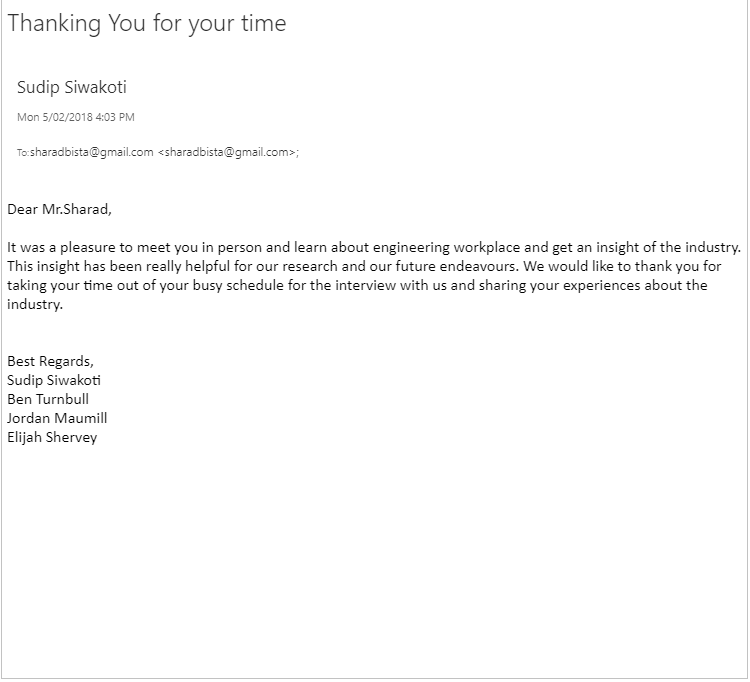
\includegraphics[height= 20cm,width=1\textwidth]{thankyou.PNG}
    \end{figure}
    
\section{Appendix 2: Interview Photo}\label{sec: Questionnaires }
\begin{figure}[h!]
	\centering
    \includegraphics[height= 5cm,width=.5\textwidth]{2.jpg}\linebreak
     
    \centering
    \includegraphics[height= 5cm,width=.5\textwidth]{3.jpg}\linebreak
   
   
    \centering
    \includegraphics[height= 8cm,width=.5\textwidth]{1.jpg}\linebreak
    \end{figure}\pagebreak

\section{Appendix 3: Engineers's Contact Details}\label{sec:APPENDIX3}

\centering
Engineers Name: Sharad Bista.\\
Email: sharadbista@gmail.com\\
Mobile: 0419238101

\end{document}